%% Document initiation %%
\documentclass[11pt]{article}
\usepackage[utf8]{inputenc}
\usepackage[a4paper, total={6.3in, 8in}]{geometry}
\setlength{\parskip}{1em}


%% Package Declarations %%
\usepackage{amssymb,amsmath, algorithm, algorithmic}
\usepackage{xcolor, times,psfrag,epsf,epsfig,graphics, tabularx, array}
\usepackage{tikz}
\usepackage{multicol, wrapfig, ctable}
\usepackage{fancyhdr, hanging, setspace}


%% Comman Declarations %%
\newcommand\mybox[2][]{\tikz[overlay]\node[fill=blue!20,inner sep=2pt, anchor=text, rectangle, rounded corners=1mm,#1] {#2};\phantom{#2}}
\renewcommand{\arraystretch}{1.2}

\pagestyle{fancy}
\begin{document}

%% Document Building %%
\graphicspath{{images/}}

%% Title %%
\title{Relativistic Runaway Electrons and Lightning Discharge: a Qualitative Overview}
\author{William Jardee}
\date{\today}
\maketitle


\begin{multicols*}{2}
    

    \noindent
{\bf \LARGE Introduction}

    One of the favorite facts many people trying to inspire young minds towards studying physics, is the concept that we have little idea of how lightning strikes actually happen (this was one of the initial curiosities that inspired me as a kid). While this is true, we do understand little about the fine details of the mechanics that drive lightning strikes, especially how they are initiated, within the last couple decades a new, promising theory has been developed to explain events like lightning initiation. I set out to begin understanding the introductory premise of two primary questions that have yet to be comprehensively answered:
    \begin{enumerate}
            \item By what physical mechanisms is lightning initiated, and how do these mechanisms related to step leaders, a known phenomena that will be explained later?
            \item What physics describes X-ray flashes and other powerful emission events seen from thunderclouds and how is this physics related to the mechanisms that initiate lightning strikes, both cloud to ground and compact intra-cloud discharges (CIDs)? 
    \end{enumerate}

    These ideas are all wrapped up in a ``rapidly expanding field of energetic particle and radiation physics in terrestrial and planetary atmospheres, and their effects" which Dwyer coined ``high-energy atmospheric particle physics." The fundamental idea was first proposed by C.T.R. Wilson in 1925 with his theory of Runaway Electrons, relativistic particles in a fluid that are able to accelerate into lower energy states. I will go over the necessity of RREs (relativistic runaway electrons) in thunderclouds, how they exponentially grow into an avalanche event with numerous feedback loops, and what type of conditions are required to allow the events to happen at all. Then, I will explore what type of photon emissions are thought to come from these RRE events and how they can be used to model step leaders. Finally I will give a quick overview of the current stance of the theory with respect to current computational models and observational data. 
    \newline
    

    \noindent
{\bf \LARGE Background Physics}

    Before we delve into Relativistic Runaway Electrons (RREs), we must first establish a base understanding of storm clouds. The simplest depiction of a storm cloud is a type of tripole, where the top, middle and bottom of cloud are charged. The typical charge distribution has about 40 coulombs of charge at the top, -40 coulombs in the middle, and 3 coulombs at the bottom (see figure 1 for a visual depiction).$^{(5)}$ Notice how this will create two net electric fields within the cloud: one pointing down towards the center and another point up also towards the center. 
    
    The process that creates this polarization isn't fully understood yet, but the primary charge transfer is thought to include collisions between soft hail, called graupel, that are heavy enough to fall in the cloud's updrafts and smaller crystals of ice that are light enough to be carried upwards. These lighter crystals give their negative charge to the graupel and then follow the updraft to the top portion of the cloud.$^{(5)}$ This process leaves the negative graupel in the center of the cloud while lifting positive ice towards the top. Along the outside surface of the cloud a thin layer of negative charge accumulates because of the conductivity of the nearby air, however this effect won't play a meaningful role in the runaway phenomena. While the charges and layout of the tripole can vary, the most typical cloud is what is drawn here and will be the basis for nearly all the theories developed. 
    
    Storm clouds discharge through many different types of lightning strikes from cloud to ground, ground to cloud, intra-cloud (inside the cloud's mass), etc.$^{(5)}$ While all strikes appear and hold some significance to the story of lightning physics, the most common ones are cloud to ground and intra-cloud strikes. Because these are the most common strikes they will be focus of our treatment.

    Lightning strikes themselves are the result of an electric breakdown in the atmospheric air between the starting and ending point. Clouds produce branches of ionized air between the cloud and the targeted surface, the most important of these branches are called step leaders. Once there is a completed path the electrons are able to flow out of the electric field and towards the earth or to another part of the cloud that has a lower potential.$^{5}$ This basic understanding will serve us well enough to understanding RREs. With a classical treatment, air observes a electrical breakdown, or dielectric breakdown, at about $E_{th}$ = 2 MV/m.${^1}$ This $E_{th}$ describes the field where the generation of new electrons from ionization surpasses the recombination rate and we get an exponential growth of free electrons. The value is derived by assuming a mean electron energy of ~2eV in air at atmospheric pressure.$^{(1)}$ This means that, from the limited classical model, a large electric field must be present at the starting location of the lightning strike to account electrical breakdown. 
    \begin{center}
        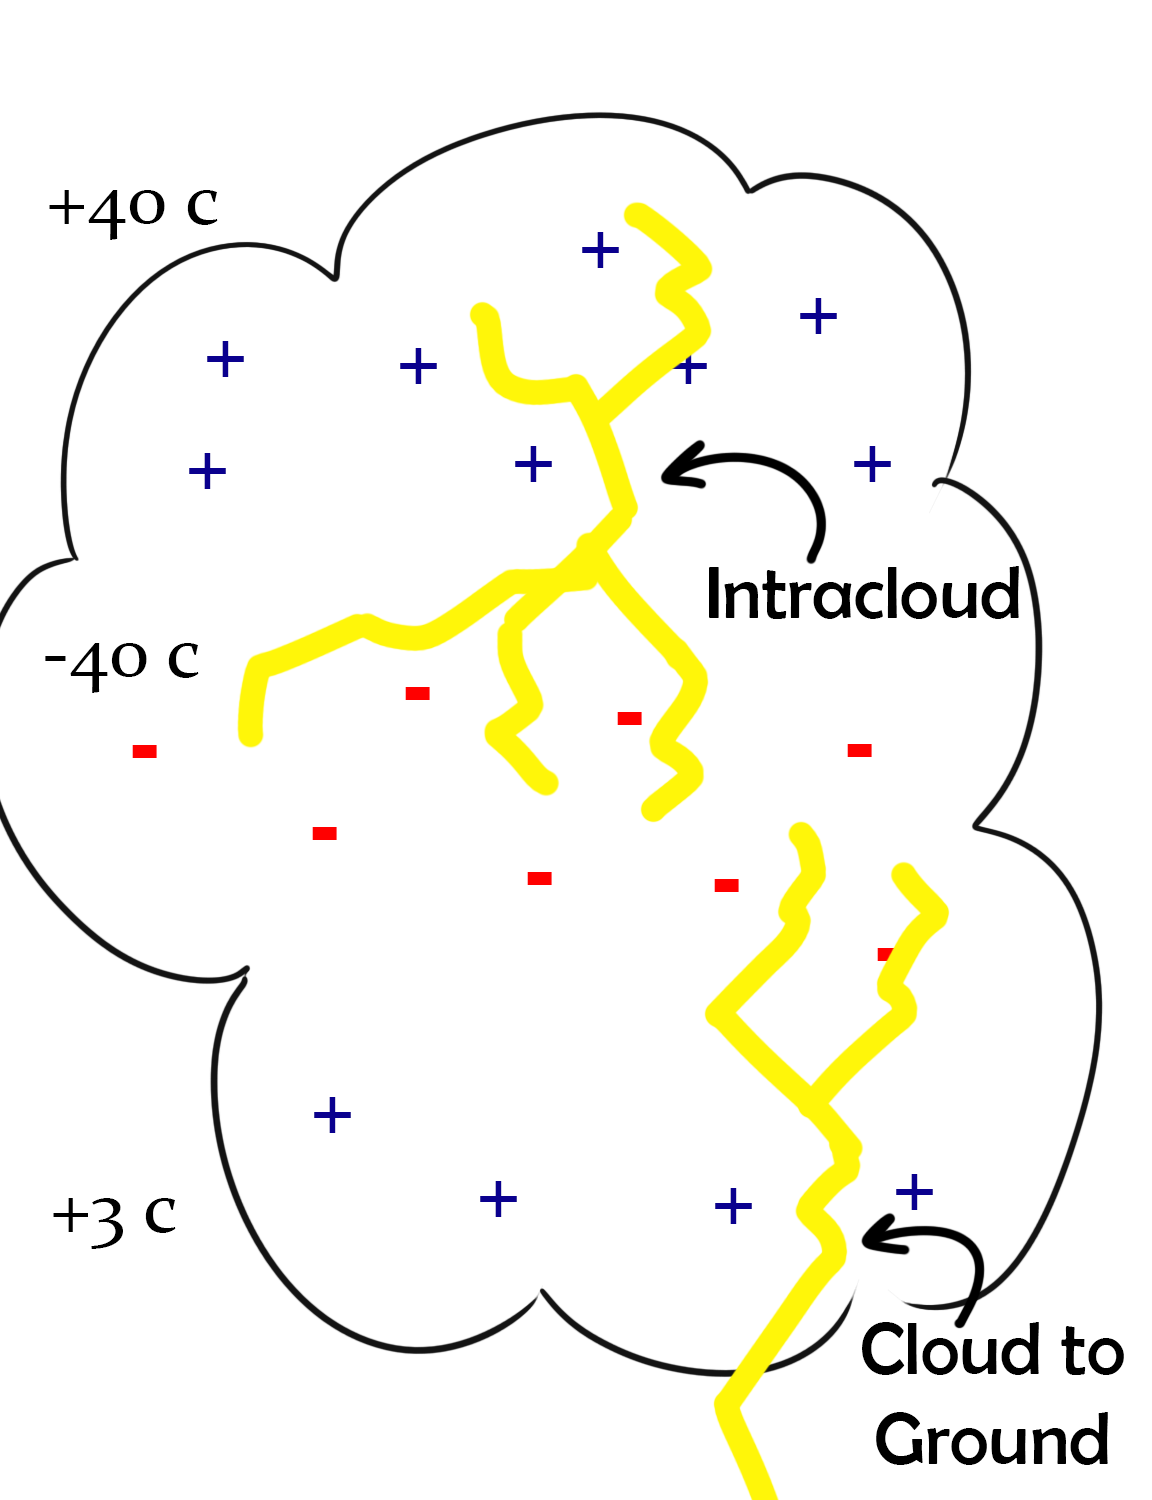
\includegraphics[width=.65\linewidth]{clouds.png}
    \end{center}
    \textbf{fig 1:} \textit{A typical charge layout of a cloud with the two most common discharge types storm clouds exhibit.}
    \newline
    

    \noindent
{\bf \LARGE Physics of RRE}
    
    Here is where we restate the dilemma that brought us to needing a relativistic theory to explain lighting propagation in the first place: how do we rationalize both the requirement of step leaders to initiate strikes, consequently needing a $E_{th}$ = 2 MV/m or 1-1.4 MV/m in heavy rain, while the maximum observed electric field in storm clouds is about 200 kV/m, a 1/10 of what we expect?$^{(1)}$ The answer is with a relativistic oddity: ``runaway electrons". As defined by Dwyer: ``when the rate of energy gain from an electric field exceeds the rate of energy loss from interactions with air then the energy of an electron will increase and it will `runaway.'"${(2)}$ 
    
    The premise behind the physics here is moderately simple to understand. As a non-relativistic particle moves freely through a gas, in this case we are considering an electron traveling through a storm cloud, the mean free path will be inversely proportional to the number density of particles in the cloud, as a less dense gas will mean less targets to rebound off of. However, if this particle gains enough kinetic energy to start moving relativistically it will enter a sweet spot where the deBroglie wavelength is comparable to the size of the particles in its way. This wavelength allows the particle to effectively ``jump" over some collisions and thus the ``friction" the particle has with the environment will start to go down. The ``friction" force is often referred to as a braking force (as it is the force slowing the acceleration from the E-field). This is what we call relativistic runaway electrons. 
    
    When these electrons collide with atoms, they can knock other electrons free through moller scattering. These newly excited electrons will have a reasonable chance to be given enough kinetic energy to start traveling realistically as well.$^{(1)}$ The number of relativistic runaway electrons then compound on an order of an exponential growth and create what is called a Relativistic Runaway Electron Avalanche (RREA). Once this avalanche reaches a significantly high speed, bremsstrahlung, other high energy interactions, and reseeding events put a limit on how much this braking force can be reduced.$^{(2)}$ Reseeding events are feedback phenomena where electrons, positrons, and photons loop around to initiate new avalanches. This idea will be touched on in a little more detail soon.
    
    \begin{center}
        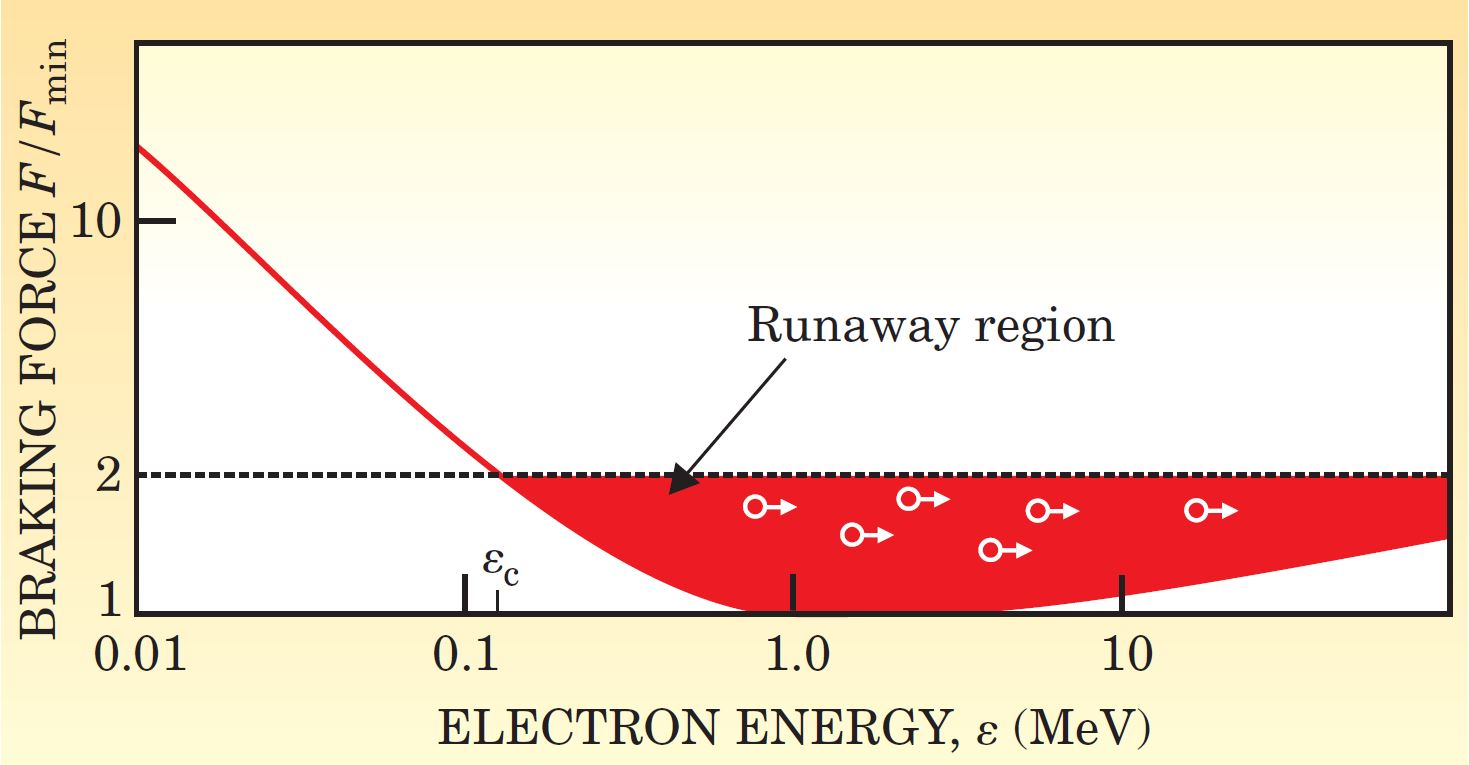
\includegraphics[width=0.5\textwidth]{images/Breaking Plot.JPG}
    \end{center}
    \textbf{fig 2:} \textit{The evolution of braking force with respect to the electron's energy in air. As the electron gains more kinetic energy it can decrease the effective force it feels until the braking force is less than the accelerating force of the electric field, at this point it is in runaway. This graph was borrowed from (1).}
    
    An RREA is a compounding growth event and must begin at some first particle. The catalyst of these events come in a variety of particles, often referred to as a seed particle. If the electric field inside the cloud is strong enough then electrons can independently reach the breaking speed, spontaneously becoming the catalyst. This field is called the breaking field $E_b$. While the electric field within clouds are usually below this breaking field, certain hot-spots can form within the field by random fluctuations and source seed particles for avalanches that exist outside of these initial hot-spots. These electrons are usually called `cold runaway' or `thermal runaway'.$^{(1)}$ Cold runaway is possible, but depend on the presence of random hot-spot in the cloud. A more reliable source comes from outside the clouds in the form of cosmic rays and radioactive decay, cosmic rays being a more likely candidate for a seed particle because of how common they are. 
    
    Cosmic rays are highly-relativistic particles traveling near the speed of light from extraterrestrial sources, like the sun.$^{(3)}$ Since these particles are traveling so quickly, they don't see much deviation from their initial velocity, which is usually straight down. In the presence of an electric field, like that of a storm cloud, these initial particles quickly decay into about $10^6$ to $10^{10}$ other particles like protons, neutrons, pions, electrons, and photons.$^{(2)}$ However, primarily through the decay of the $\pi^0$ into two photons that travel nearly horizontally in order to conserve vertical momentum, the cosmic ray dissolves into a mirage of particles traveling mostly vertically with a large transverse footprint.$^{(1)}$  These interactions produce a pancake type shape a couple meters tall and about 100-150 meters across.$^{(2)}$
    
    According to extensive monte carlo computations, this phenomena, called a Cosmic Ray Extensive Atmospheric Shower (EAS), produces about 89\% are protons, 10\% electrons, and 1\% other particles in the first generation of products.$^{(4)}$ More particles are created in subsequent generations and some have tried to use these random fluctuations as a reasoning behind some of the high energy events seen in storm clouds. However, running monte carlo models allowing for both first and second generation Cosmic Ray EAS, the energy added by the second generation is negligible compared to the first.$^{(4)}$ A primary reason to this is that the EAS loses energy as the particles fall through the atmosphere, causing fewer high energy collisions. All the interactions considered in the computational and theoretical analysis of RREA only include electrons, so the number of actual seed candidates are a magnitude lower than the total created, $10^5$-$10^9$. I haven't been able to find a concrete reason as to why models only cite electron interactions; however, from my reasoning it must be because a) the electron have a charge that prefers to fall towards the earth in the electric field and b) all other popular particles, like the neutron and proton, are much heavier, so they will not be able to reach this runaway speed in the same electric field. 
    
    When an EAS is considered in the presence of a storm cloud, the number of particles created and the energy of said particles are considered as a Runaway Breakdown Extensive Atmospheric Shower (RB-EAS). A comprehensive derivation of the theoretical framework of RB-EAS was first developed by Gurevich in 2004. The key takeaway of the phenomena was that the number of relativistic seed particles grew very quickly when the electric field of the cloud was slightly larger than the observed electric field threshold of lightning initiation. With just a 0.4 increase in the electric field the number of seed particles grows by $10^4$ between $E_{max}/E_c =1.2$ to $E_{max}/E_c =1.6$ and $10^2$ between $E_{max}/E_c =1.6$ to $E_{max}/E_c =2.0$. In the graphs we can see a bias in number of seed particles towards higher altitudes. As seed particles fall through the cloud they are more likely to interact in a way that removes their energy, either by dissipation or by an RREA event. Consequently, the farther down the cloud we are the fewer particles will continue to weave between collision partners. With a higher E-field these interactions are more likely to happen at higher energies, removing more energy from the EAS in a shorter time. The energy that the particles gain has a strong relationship with the magnetic field strength. Further, if the energy that the electric field gives to all these seed particles is calculated, the energy quickly blows up.  When the maximum electric field is 1.05-1.20 times the $E_c$ the energy that the particles gain from the electric field in runaway is 6-100 that of the seeding cosmic ray's energy. When the electric field is 1.4-1.6 times $E_c$ the energy gained jumps to $10^3$-$10^5$ the seed particle's energy.$^{(6)}$
        
    Through Monte Carlo calculations, the threshold field for the a RREA was $~E_c$ = 2.83 V/m $\times n$, where $n$ is the density of air at sea level.$^{(2)}$ We see that his value is about $130\%$ that of the breaking field. The $E_b$ value was determined as if our electron was traveling directly on the electric field lines. For most particles, however, this not the case, and through careful consideration of the angles in the theory the field inflates by a factor of $0.3$.$^{(6)}$ When compared against observational data, this $E_c$ to $E_b$ describes the upper and lower limits of the electric fields right before lightning strikes.$^{(1)}$
    
    \begin{center}
        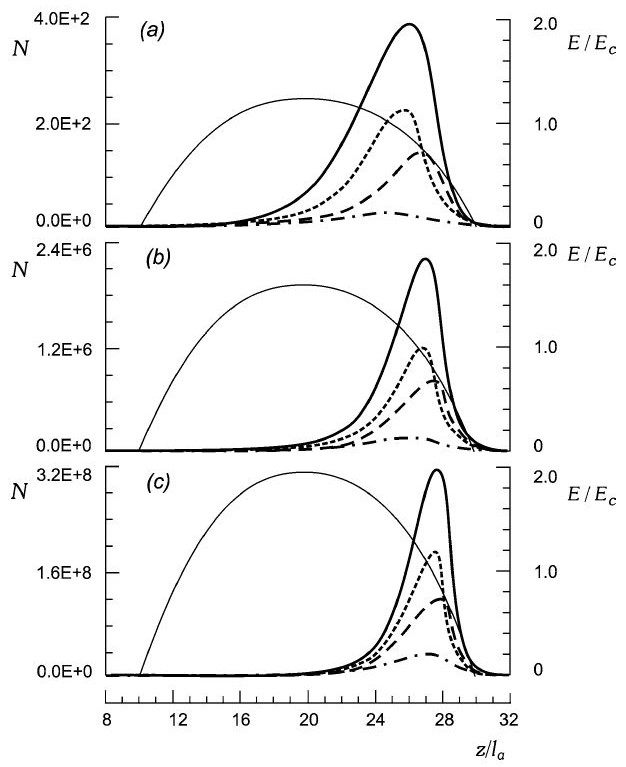
\includegraphics[width=0.95 \linewidth]{images/Dependence on relativistic electrons plot.JPG}
    \end{center}
    \textbf{fig 3:} \textit{The number of present relativistic EAS secondaries present as a function of a scaled height factor, $z/l_a$, more details about this scale can be found in the source. The $\delta$ parameter is (a) $\delta = 1.2$, (b) $\delta = 1.6$, (c) $\delta = 2.0$. The thin line shows the electric field, dashed line relativistic electrons in energy interval $1< \gamma <3$, point line $3< \gamma < 10$, dashed-point line $10< \gamma <100$, solid line is the total number of relativistic electrons. This graph was borrowed from (6).}
    
    Once a RREA is in action they will propagate until they reach a steady state. There are various characteristics used to describe this state, the rate of avalanche production, the length of the avalanches, the total energy of the avalanche, both as a maximum and an average. All of these properties can be used to analyze the behavior, but the simplest is to look at the average avalanche length. This avalanche length is the result of an unstable feedback loop. While traveling, the electron loses energy to what we called the braking force earlier. This braking force is primarily a combination of ionization and atom excitation, and moller scattering. These interactions, along with background from CR-EASs, introduce a photon rich environment that allows for an abundance of compton scattering, the photoelectric effect, pair production and rayleigh scattering. 
    
    When the photon is of relatively low energy, up to 100keV, the primary interaction will be the excitation of atoms and electrons in the form of the photoelectric effect, where the photon is absorbed and unable to cause any more interactions. When the photons have 100keV to several MeV there is enough energy to cause compton scattering. After accounting for subsequent interaction right after the initial production, Compton scattering provides photons with an energy of about 100keV.$^{(5)}$ If the photon has a significantly high energy, then the photon can undergo pair production, creating an electron and a positron. We focus on a $e^- + e^+$ production because it will allow us to create a reseeding event through an annihilation higher in the cloud. If we allowed for creation of a $\mu + \overline{\mu}$, then we wouldn't be allowed to interact with electrons higher in the cloud except in a scattering interaction, which would send the collided electron back upwards, the opposite direction of a RREA.
    
    Each of these interactions will be occurring abundantly when significant energy is present, but the most notable at each tier will be the interaction that allows for the most dramatic changes. As energy increases the dominant interaction will be the photoelectric effect, then compton scattering, and finally pair production. Notice that rayleigh scattering, or elastic scatting of light off particles much smaller than the wavelength of the light, is not seen as a notable interaction. That is because the elastic scatting only redirect photons, and thus has little effect on the state of the avalanche other than to increase the distribution of photons. 
    
    In the first case, if compton back-scattering happens, the photon can be ejected so that it reenters the avalanche area and is able to excite an electron that will be able to act as the seed particle to another avalanche. In pair production, the positron follows the electric field in the opposite direction of the electronic avalanche until it get outside of the avalanche area, where it is able to interact with thermal electrons and start another avalanche through Bhabha scattering.$^{(2)}$ When considering these feedback loop, it is easy to see that the number of avalanches in a moderately sized electric field, will grow on the order of an exponential. These positive feedback loops are very unstable. According to monte carlo calculations with our most recent model of RREAs, the average energy of the runaway electrons in this steady state is ~7 MeV.$^{(2)}$ The large flux of escaping photons from compton scattering and bremsstrahlung in these chain reactions have been proposed as the source of Terrestrial Gamma ray Flashes (TGFs), but more on that later. 
    \newline
    

    \noindent
{\bf \LARGE Emissions and Step Leaders}
    
    One of the first applicable uses of RREA theory is how Cosmic Ray EAS initiate short lived RREA to create Narrow Bipolar Events (NBEs). When the electric field inside a storm cloud cannot properly fuel the exponential type growth of the number of avalanches, RREAs created from Cosmic Ray EAS seeds are short lived with a lifetime on the order of $\mu s$.$^{(2)}$ These quick fluxes of electron flow give pulses of current that grow on an exponential order, but the unstable avalanches then decay at an an similar rate. Gurevich has a derivation of the mechanism behind this growth: the current rise time, the time spent increasing the number of electrons in the RREA, is inversely proportional to the density of air, which is related to the inverse exponential of altitude; $t_r \propto \frac{1}{N_{air}} \propto e^{z}$. Similarly, the discharge time is inversely related to the square of the density; $t_r \propto \frac{1}{N^2_{air}} \propto e^{2z}$.$^{(6)}$ 
    \begin{wrapfigure}{l}{0.2\textwidth}
        \centering
        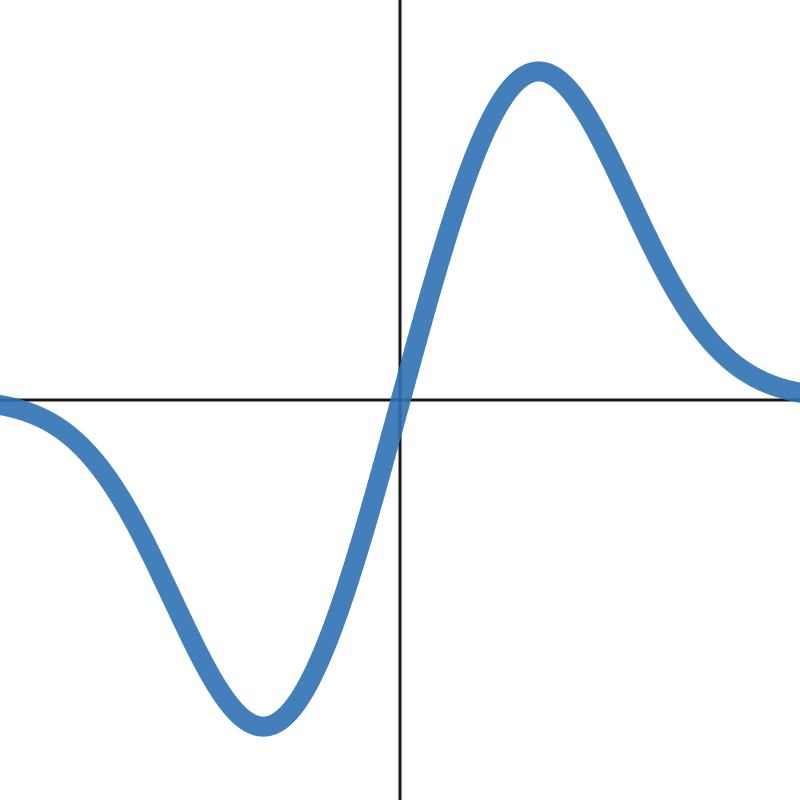
\includegraphics[width=0.2\textwidth]{images/desmos-graph.png}
        \textbf{fig 4:} \textit{A bipolar spike.}
    \end{wrapfigure}
    This rise-fall behavior will be mirrored after the RREA is done as the now positive region redistributes electrons to neutralize the area. This gives a very strong radio bipolar spike that have been observed to only last a couple $\mu s$, which is in good agreement with the theory.$^{(1)}$ These strong spikes are in same frequency as many power grid components and atmospheric devices observational devices, making interference a common occurrence.
    
    It has been proposed that when the avalanches exist in an environment supporting exponential growth, the sudden flux of photons can source terrestrial gamma ray events. There are two flavors of these events: long emission with a time scale in the seconds, called Gamma-ray glows, and short emission with time in the $\mu s$ range, called terrestrial gamma ray flashes (TGFs). As feedback events happen in the propagation of RREAs, a fraction of these photons will be leaked out of the storm cloud and describe a glowing event around clouds.$^{(1)}$ These glows exist in the blue region of the visible specta and have been known about long before the science of RREAs was invented. A standing issue with this theory is that the observed photon wavelengths from glows are considerably lower than what would be created by RREA. The theory behind RREA seems to explain part of the flux coming from thundercloud glows, but it fails to fully explain the phenomena.$^{(2)}$ The short emission flashes seem to be well defined by RREA, however. In the microseconds leading up to a lightning strike a quick spike in the x-ray spectrum is observed; these are TGFs. To properly explain how the theory explains these flashes we much take a detour to talk about RREAs and the step leader model.
    
    \begin{center}
        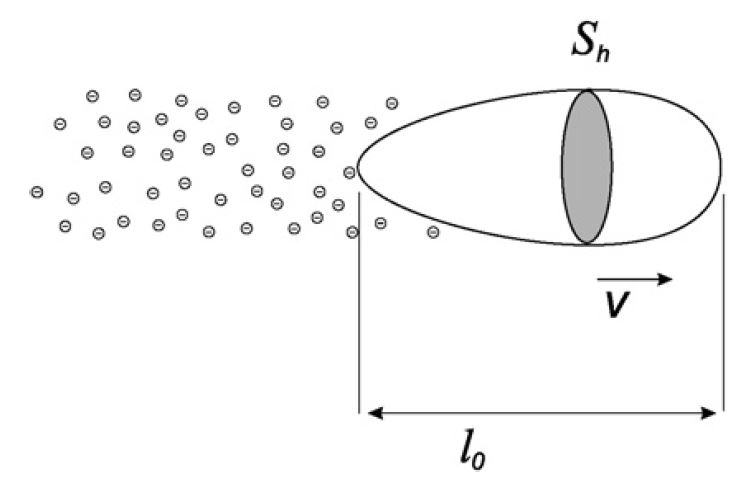
\includegraphics[width=\linewidth]{images/step leader.JPG}
    \end{center}
    \textbf{fig 5:} \textit{A depiction of Gurevich's SRB step leader model. The tear drop gets its shape from a collection of conventional breakdown effects and runaway effects. The calculated dimensions of the head are $S_h = 1-10 cm^2$, $l_0 ~ 10 cm$, $\Vec{v} \approx 6 \times 10^7 cm/s$. It should be noted that the values presented here do not agree well with laboratory observations that place $S_h ~ 10^{-2}$, this is because lab created step leaders are the product of a more forced/higher energetic process and are not detected well. All these numbers and graphics were created by (7).}
    \newline
    
    In lightning propagation, stepped leaders are an region of air that has experience a breakdown prior to the complete lightning path. These paths can be seen optically right before a lightning strike; they look like smaller branches coming off the primary strike. These leaders are seen is discrete steps progressing in a branching pattern towards the target, until eventually they meet either the surface or leaders coming off this surface. The edge of these branches, stepped leaders, are called step leaders (fun terminology, I know). The actual theory and details expand well beyond this, but the idea of a tree made up of discrete steps of pockets of air already exhibiting breakdown will serve us well enough.
    
    RREAs are thought to be one of the main initiators in the process of lightning strikes by helping providing step leaders. Gurevich proposed a theoretical framework of how runaway breakdown can exist in a strong electric field, where this field can form a teardrop like structure (see figure 4) to guild leader lines.$^{(7)}$  The specifics about the dimensions of these teardrops can be see in that paper, but the important takeaways is the energy of particles and the leader's speed. In the strong electric field region created with step leaders the particle energies are 2 to 4 times the magnitude of the regular energy of runaway electrons. This large flux of electrons, and the strong magnetic field that travels with them, is about 70-100 times the breakdown field of air and is thought to be able to initiate a breakdown of air in a lightning strikes.${^{(7)}}$ Since these step leaders are created from avalanche effects, their speed is limited by the speed of the avalanche speed, this becomes even more important if we think about the feedback effects happening in parallel with the movement. Dwyer does point out an issue with this theory: that the avalanche time scale described in this theory, which is proportional to $\delta^{-2/3}$, where $\delta$ is the maximum E-field in the region over the threshold field ($E_{max}/E_c$), conflicts with the currently accepted observed relationship to $\delta^{-1}$. This fact does skew a couple key numbers, and the whole process is still not fully understood, but the working model assumes that feedback events puts an upper limit on this avalanche lifetime and still accepts the hypothetical frame work that Gurevich proposed.$^{(2)}$
    
    It is seen that step leaders drastically slow down in the first 15-20ns after their creation.$^{(2)}$ TGFs are a probably explanation of this phenomena. As the energetic blob of electrons moves, it quickly radiates a pulse of x-ray photons that are seen before lightning strikes.$^{(4)}$ It is important to note that TGFs are only an intra-cloud (strikes inside a thundercloud) event, as it has been conclusively shown that TGFs propagate upwards from the middle negative charge to the positive top charge of a cloud. Because of the high altitude these TGF events occur at, they were not explainable by EMP or slowly varying electric fields, which are not considerable mechanisms in large thunderclouds.$^{(2)}$ All these physical theories are quite convincing, however it should be remembered that the exact physical processes occurring during the initial upward leader propagation in an IC light flash is far from understood. Furthermore, the idea of RREA has been applied to explain other flashing events that happen lower in the cloud and in other strike types, i.e. cloud to ground, but have not provided a convincing theoretical framework yet.
    \newline


    \noindent
{\bf \LARGE Observational Data}

    \quad The first production method to test RRE was done by Lehtinen in 1999, leaning almost exclusively on Moller scattering.$^{(1)}$ While the process showed good proof on concept, the model neglected to involve bremsstrahlung interactions along with many other electron interactions that would show to be crucial to explaining the processes. Within the next five years two Monte Carlo codes were written, the REAM (Runaway Electron Avalanche Model) and ELIZA by separate atmospheric physics groups. These programs introduced many interactions that were thought to be influential to the production of runaway electrons and RREAs. The current model of the codes include a laundry list of interactions:
    
    \begin{itemize}
    \setstretch{.5}
    \item Runaway electrons
        \item Moller scattering
        \item Elastic scattering with coulomb shielding
        \item Bremsstrahlung production of x-rays and $\gamma$-rays and their subsequent interactions:
        \begin{itemize}
            \item Photoelectric effect
            \item Compton scattering
            \item Pair production
            \item Rayleigh scattering
        \end{itemize}
        \item Bhabha scattering
        \item All the above interaction with their positron counterparts$^{(1)}$
    \end{itemize}
    \setstretch{1}
    What I provided just now is not a fully comprehensive list, but provides the most notable interactions that are have the largest impact on the simulations. 
    
    A common error in running these simulations and developing theory is to not apply proper limits in accordance to the physical setup. Dwyer puts it colorfully when he says many theorist have "cranked up the high-voltage knob" and applied the theory of RREAs where it doesn't belong.$^{(1)}$ As we covered earlier, different processes become dominant with different physical conditions. For example, when talking about interactions with air compton scattering dominates in the mid regime while pair production dominates in the higher energy regime. But, when all these conditions are considered carefully, the produced avalanche length, avalanche lifetime, electric field threshold, RRE speeds, and diffusion coefficients all agree well with the observed data.$^{(2)}$
    
    One of the reasons our understanding of high-energy atmospheric particle physics is so limited at this point is because of the lack of good observational data. Until modern computing, theorists relied on observed data to give a basis of new ideas and questions. With Monte Carlo and other simulation techniques that problem has been partially mitigated, but it doesn't solve the issue that we are trying to use extremely sensitive instruments to measure finite phenomena in an incredibly messy electro-magnetic environment. Through the tiresome analysis of scientist in the past, what we have been able to deduce from observational data is that RREA can only be part of the bigger picture here. Through the ionization effect of RREA, the theory can only account for about 1/10 of the total current needed to initiate a lightning strike. A proposed possible correction to this value is to consider high and low energy electrons as one population, instead of separate events.$^{(2)}$ The current theory models different tiers of electron energies (thermal electrons, those blow 100keV, those below several MeV, and those above several MeV) as mostly separate events running in parallel. The theories also divide weak and strong magnetic fields as two different stages of the process instead of allowing the two fields to interact. Once these processes are all mixed together in one algorithm, the computation time grows to an unreasonable duration. 
    
    Another barrier of work, and a primary reason our understanding of the exact processes is so limited, is that RREAs cannot be studied in the lab setting. When Wilson first brought up the idea of runaway electrons, specifically with regards to atmospheric physics, he had developed the cloud chamber for observation of this phenomena. The length scale of avalanche multiplication is on the order of hundreds of meters, which is not a feasible lab setting for a setup like a cloud chamber.$^{(5)}$ While smaller discoveries, like gamma ray flashes in smaller RRE events, have been investigated with some success, running trials on systems as large as storm clouds is outside the real for anything but a digital medium. 
    \newline
    

    \noindent
{\bf \LARGE Conclusion}
    
    Surveying the theory and computational analysis of runaway breakdown with respect to relativistic runaway electron avalanches provides some hope in the subject of high-energy atmospheric particle physics. We saw that when electrons are able to reach a high enough velocity that their momentum allows them to seemingly ``jump" over opposing collisions. The source of these initial high energy electrons can either be through cold runaway, when a pocket of E-field is high enough to accelerate an electron to this threshold speed, or a seeding particle introduced by extensive atmospheric showers or radioactive decays. Once the electron is traveling relativistically, their effective braking force begins to drop to below the force of the electric field present in a storm cloud and they are allowed to accelerate downwards. These relativistic electrons are able to multiply directly, by collisions with other electrons, and indirectly, by production of photons through bremsstrahlung and moller scattering. In turn, an ``avalanche" of electrons is creates and named a relativistic runaway electron avalanche. The photons and positrons created in this mess of an avalanche are able to loop around are create an unstable feedback loop, essentially forming an avalanche of avalanches. The steps to creating the RREAs can be summed up in the folowing steps:
    
    \begin{enumerate}
        \item Inhomogeneous characteristics of thunderclouds allow random cells of E-field above the break-even field of RREs to move around the cloud
        \item Seed particles enter the thundercloud, either by CR-EASs or by random excitation of a particle in the moving field
        \item These seeds allow for RREAs to begin, and are feed by positive feedback loops
        \item Some stochastic mechanics, partially described by our step leader model, allows for a discharge to occur
        \item repeat 1-4 with a random chance
    \end{enumerate}

    RREAs have been used to explain narrow bipolar events, storm cloud glows, terrestrial gamma-ray flashes, and step leaders. NBEs and TGFs seem to be well described by the phenomena, while glows and step leaders both seem to qualitatively line up with reality but only describe a fraction of what is actually observed. Currently, most of our understanding is coming from robust monte carlo codes, but a lot can be done to improve our understanding. Our understanding of the current physics in limited by good observational data, as the environment to collect the data is either too far away and sees too much outside noise, or is too close and tends to be overwhelmed by the amount of information provided to it. 
    

% General take away from the theory? IC NBEs (strongest radio event on earth) and TFGs are well explained by it... that's about it other than good theory

% Applications of this: understating how lightning works, further understanding of RREA for fusion reactors, understand radiation emission events to protect air/space craft (dosage idea),

\end{multicols*}


    \newpage
    \noindent
{\bf \LARGE References}\\
\setlength{\parskip}{0em}


    \begin{hangparas}{.25in}{1}
    1. A.V. Gurevich, K.P. Zybin, Physics Today 58, 5, 37 (2005); doi:10.1063/1.1995746\\
    
    2. J.R. Dwyer, D.M. Smith, S.A. Cummer, Space Sci Rev (2012) 173:133–196; doi:10.1007/s11214-012-9894-0\\
    
    3. B.E. Carlson, N.G. Lehtinen, U.S. Inan, J. Geophys. Res 113 (2008) 10307; doi:10.1029/ 2008JA013210\\
    
    4. A. Chilingarian, S. Chilingaryan, \emph{et. al.}, Sci Rep. 2017 May 2;7(1):1371. doi: 10.1038/s41598-017-01288-0\\
    
    5. J.R. Dwyer, M.A. Uman, Phy Rep. 534, 4, 147-241 (2014); doi: 10.1016/j.physrep.2013.09.004\\
    
    6. A.V. Gurevich, Yu.V. Medvedev, K.P. Zybin, Phys. Lett, A 329, (2004) 348-361;\\ doi:10.1016/j.physleta.2004.06.099\\
    
    7. A.V. Gurevich, K.P. Zybin, Yu.V. Medvedev, Phys. Lett, A 361, (2007) 119-125;\\ doi:10.1016/j.physleta.2006.05.063\\
    
    8. N.S. Khaerdinov, A.S. Lidvansky, V.B. Petkov, Atmo. Res 76 (2005) 346-354;\\ doi:10.1016/j.atmosres.2004.11.012\\
    \end{hangparas}

\end{document}
